\documentclass[landscape,a0,final]{a0poster}
\usepackage[dvipsnames,svgnames]{xcolor}
\usepackage{tikzposter} % here most of the things are defined
\usepackage{minted} %code highlighting, not working yet
% change parameters only after this line You can also start a new column with an arbitrary 
% x-coordinate by specifying explicitly the coordinate of the new block node as follows:
\usepackage[utf8]{inputenc}
\usepackage{wrapfig}
\usepackage{url}

% For blibliography styling
\usepackage{natbib}

%Used for better control on code display

\usepackage[margin=\margin cm, paperwidth=197cm, paperheight=100cm]{geometry}

% \setbackgrounddarkcolor{ForestGreen!70!black}
% \setbackgroundlightcolor{YellowGreen!90!}

% \setfirstcolor{YellowGreen!80!}
% \setsecondcolor{gray!80!}
% \setthirdcolor{red!80!black}

\title{Water Dynamics in Fogera and the Upper Blue Nile\\Farmers perspectives and remote sensing\\}
\author{Yann Chemin, Mengistu Dessalegn, Jayne Curnow\\
\bigskip
\\ International Water Management Institute}

\usetemplate{1}
\setinstituteshift{1}

\setblocktitleheight{2}
\setblockspacing{1}

\begin{document}
\ClearShipoutPicture
\AddToShipoutPicture{\BackgroundPicture}
\noindent
\tikzstyle{every picture}+=[remember picture]
\begin{tikzpicture}
\initializesizeandshifts
\titleblock{120}{1}
% \setblocktitleheight{1}
\addlogo[north west]{(2,-1)}{9cm}{./svg_images/Grass_GIS.pdf}
\addlogo[north west]{(13,-3)}{19cm}{./svg_images/OSGeo_logo.pdf}
\addlogo[north east]{(-2,-4.5)}{30cm}{./images/CR10583_1wle-iwmi_logo}

%%%%%%%%%%%%%%%%%%%%%%%%%%%%%%%%%%%%%%%%%%%%%%%%%%%%%%%%%%%%%%%%%%%%%%%%%%%%%%%%
\blocknode{Abstract}{
\noindent This research work is about finding the connection between farmers perspectives on changes of water conditions in their socio-agricultural environment and satellite remote sensing analysis.\newline\linebreak
Key informant surveys were conducted to investigate localised views on water scarcity as a counterpoint to the physical measurement of water availability. Does a numerical or mapped image identifying water scarcity always equate to a dearth of water for agriculture? To push the limits of the relationship between human and physical data we sought to ground-truth GIS results with the practical experience and knowledge of people living in the area.\newline\linebreak
\noindent We data-mined public domain satellite data with FOSS (GDAL \cite{GDAL}, GRASS GIS \cite{neteler2012grass}) and produced water-related spatio-temporal domains for our study area and the larger Upper Nile Basin.\newline\linebreak
Accumulated remote sensing information was then cross-referenced with informant’s accounts of water availability for the same space and time. During the survey fieldwork the team also took photographs electronically stamped with GPS coordinates to compare and contrast the views of informants and the remote sensing information with high resolution images of the landscape.\newline\linebreak
We found that farmers perspective on the Spring maize crop sensitivity to variability of rainfall can be quantified in space and time by remote sensing cumulative transpiration. A crop transpiration gap of 1-2.5 mm/day for about 20 days is to be overcome, a full amount of 20 to 50 mm, depending on the type of year deficit. Such gap can be overcome, even by temporary supplemental irrigation practices, however, the economical and cultural set up is already developed in another way, as per seasonal renting of higher soil profile water retention capacity fields.
\newline\linebreak
}

%%%%%%%%%%%%%%%%%%%%%%%%%%%%%%%%%%%%%%%%%%%%%%%%%%%%%%%%%%%%%%%%%%%%%%%%%%%%%%%%
\blocknode{Transpiration of Fogera crops}{
\smallskip
\begin{center}
	\begin{tabular}{p{0.5\textwidth} p{0.4\textwidth}}
	 \raisebox{-0.95\totalheight}{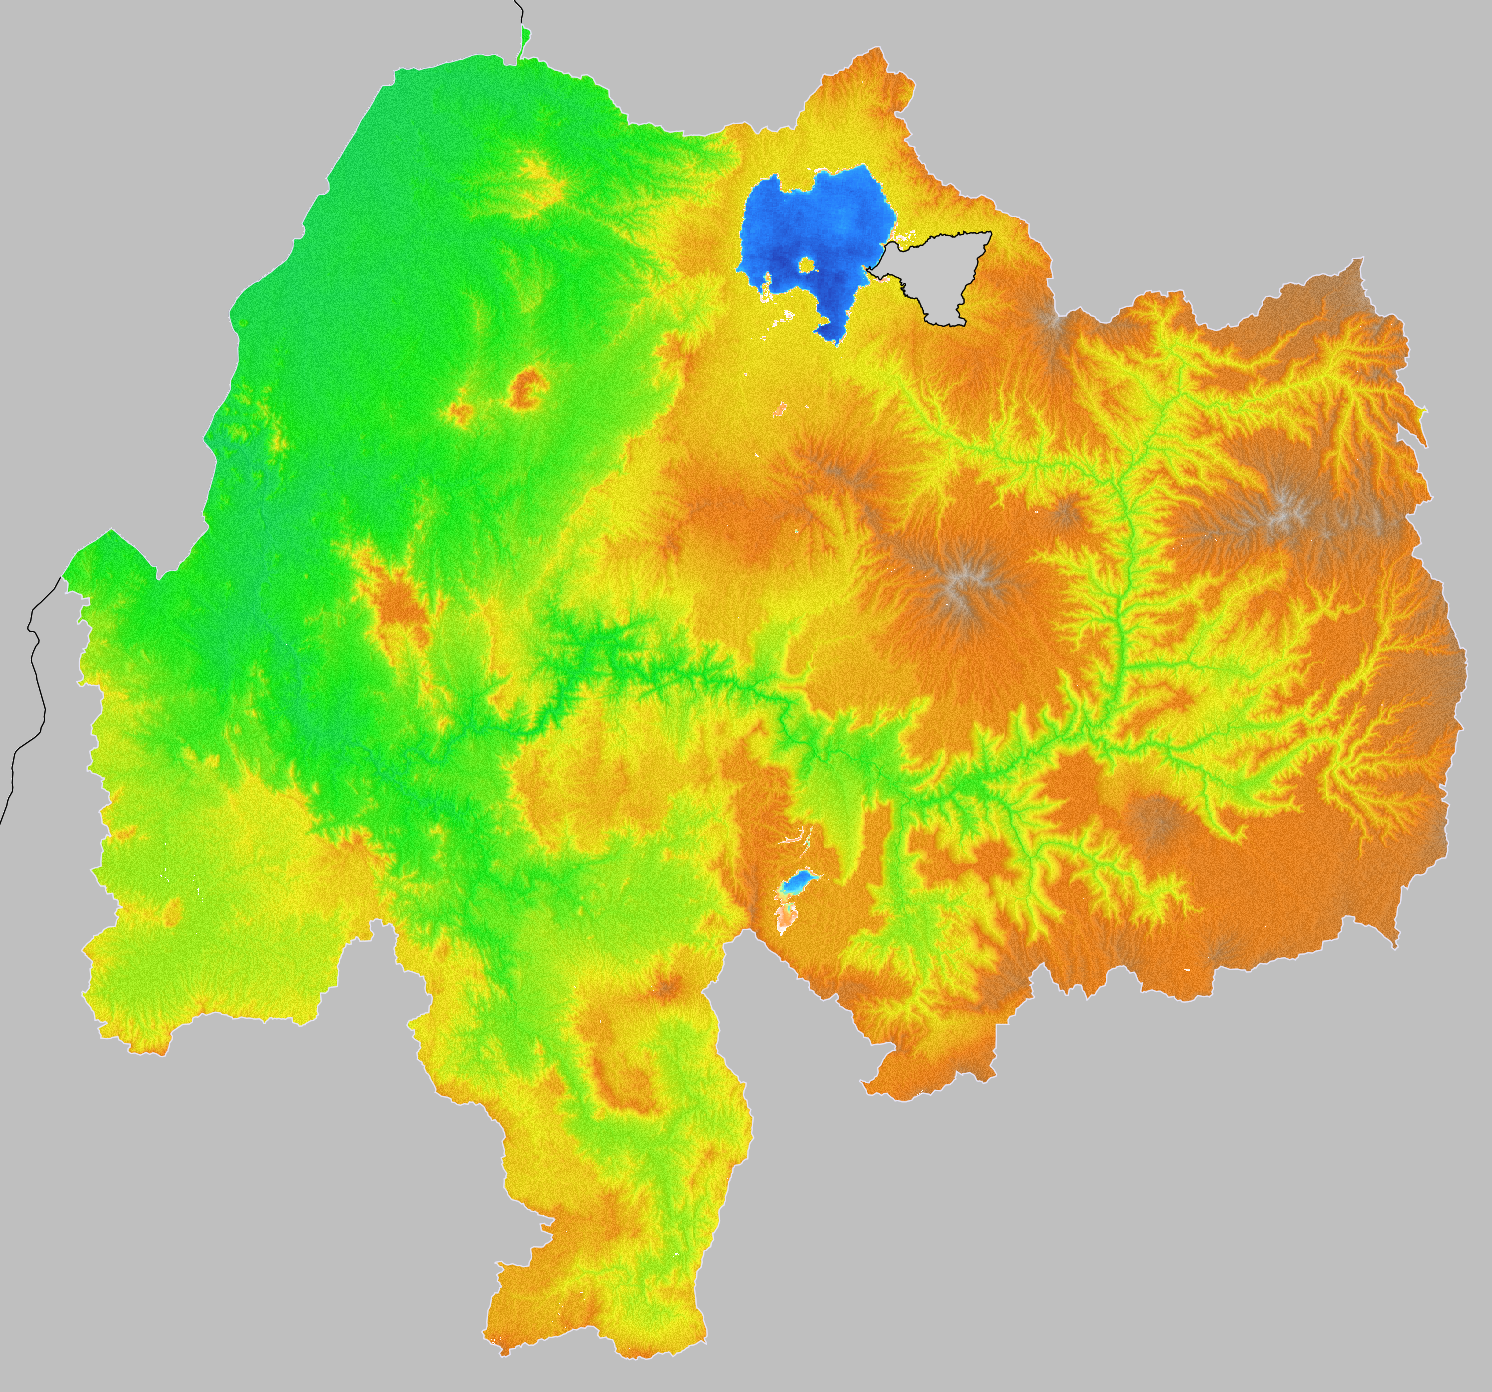
\includegraphics[width=0.5\textwidth]{./images/ETH_UBN_Fogera}}
	 \newline\linebreak
	 Figure 1: Fogera woreda location near Lake Tana.\newline\linebreak
	&
	The transpiration data in the administrative unit of Fogera (woreda) is created from the energy balance modelling \citep{chemin2012distributed} modules (i.eb.*, i.evapo.*) within GRASS GIS \cite{neteler2012grass} version 7, by partitioning the net radiation (r.sun) into soil heat flux (i.eb.soilheatflux), sensible heat flux (i.eb.h\_*) and the residual being the energy needed to evaporate water (i.eb.evapfr, i.eb.eta). This information is then fractionated into biotic (transpiration) and abiotic (evaporation) parts using vegetation fraction.\newline\linebreak
	The accumulated transpiration is subjected to temporal scrutiny, the major transpiration peak every year is preceded by a temporary increment in transpiration. This temporary change may (or not) carry enough transpiration to crop Spring maize in Fogera, the topic of this research.\newline
	\end{tabular}
\end{center}
\begin{center}
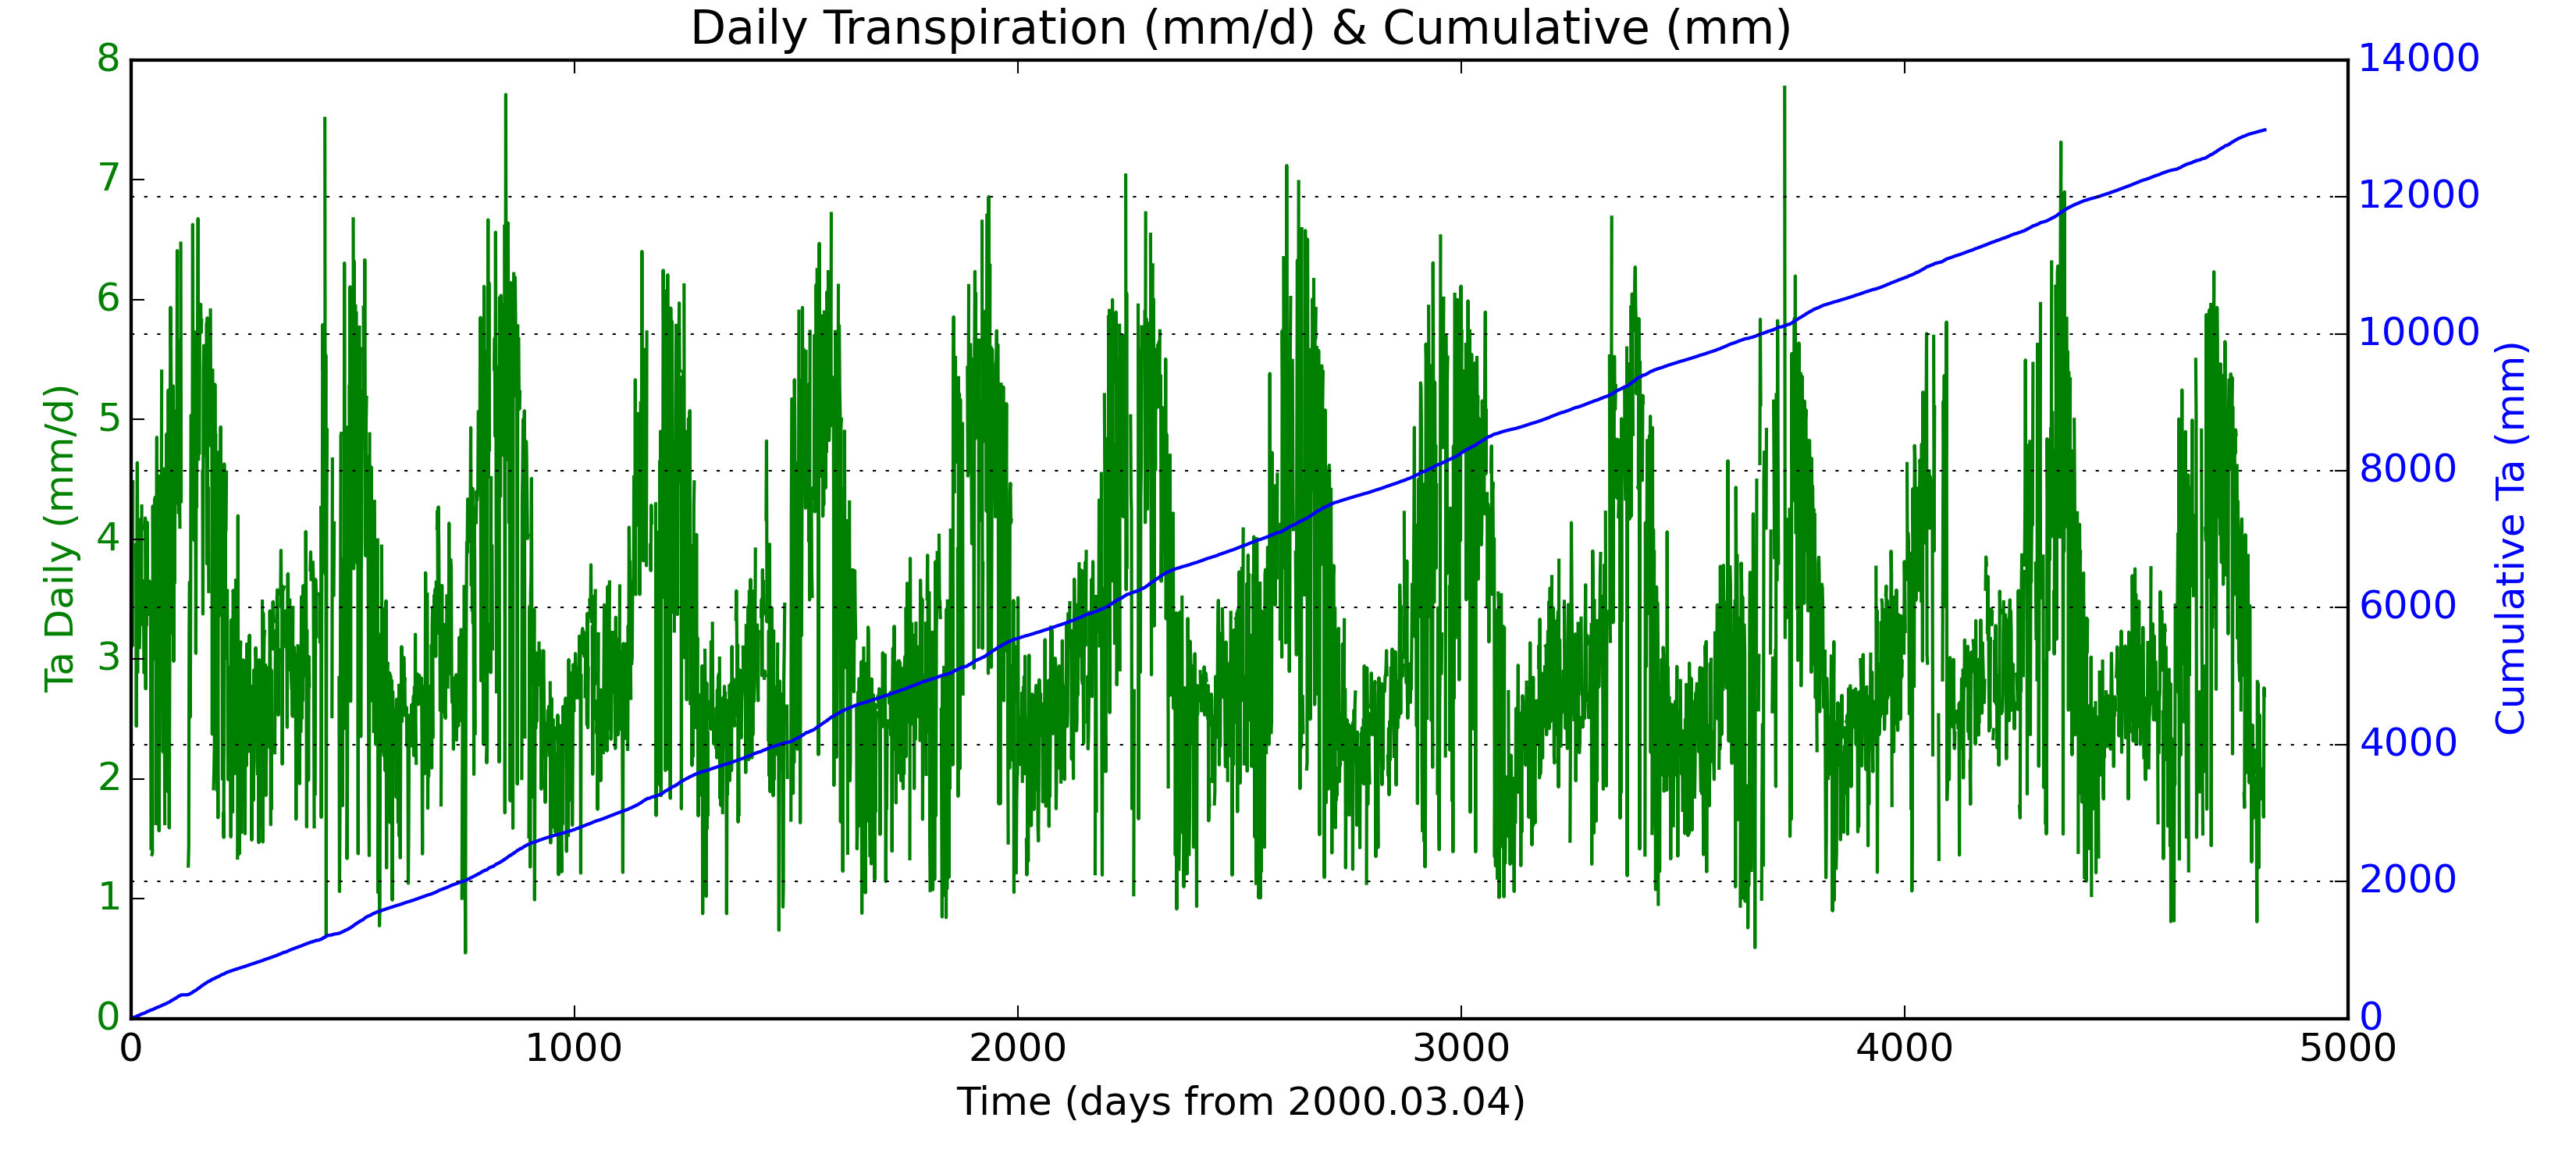
\includegraphics[width=\textwidth]{./images/Ta}
\newline
Figure 2: 14 years of daily transpiration for Gumura basin in Fogera woreda.
\newline
\end{center}

}

\startsecondcolumn


%%%%%%%%%%%%%%%%%%%%%%%%%%%%%%%%%%%%%%%%%%%%%%%%%%%%%%%%%%%%%%%%%%%%%%%%%%%%%%%
\blocknode{Farmer's perspectives on changes of water conditions}{
\smallskip
Farmer’s perspectives on changes of water conditions is tied to the socio-agricultural environment. Localised views on water scarcity is a counterpoint to the physical measurement of water availability.\newline\linebreak
Scholars have raised the concern that conventional approaches are driven largely by biophysical crop data, disregarding farmers’ behaviours, responses and strategies \citep{hurd2008challenges}. Likewise, the persistent view that risk should be determined “scientifically” and “objectively” relegated community perceptions and assessments to be uninformed, false, illusory, or irrational \citep{oliver1996anthropological}. This study aims at listening to people's perspectives and support it from remote sensing.\newline\linebreak
The practical experience and knowledge of people living in an area is driving decision-making and is a lever for assessing improvement of social and economic well-being.\newline
Farmers in Fogera, Ethiopia depend on rainfed agriculture for their livelihoods using ox-drawn ploughs. Crop production largely depends on mono-modal rainfall which starts in May and extends from June to September. The wet season crop calendar, i.e. planting and harvesting, starts in May (Blue squares) and ends by December (Red squares), depending on the type of crop (see Table 1).
\begin{center}
Table 1: Crop calendar for Fogera woreda.\newline
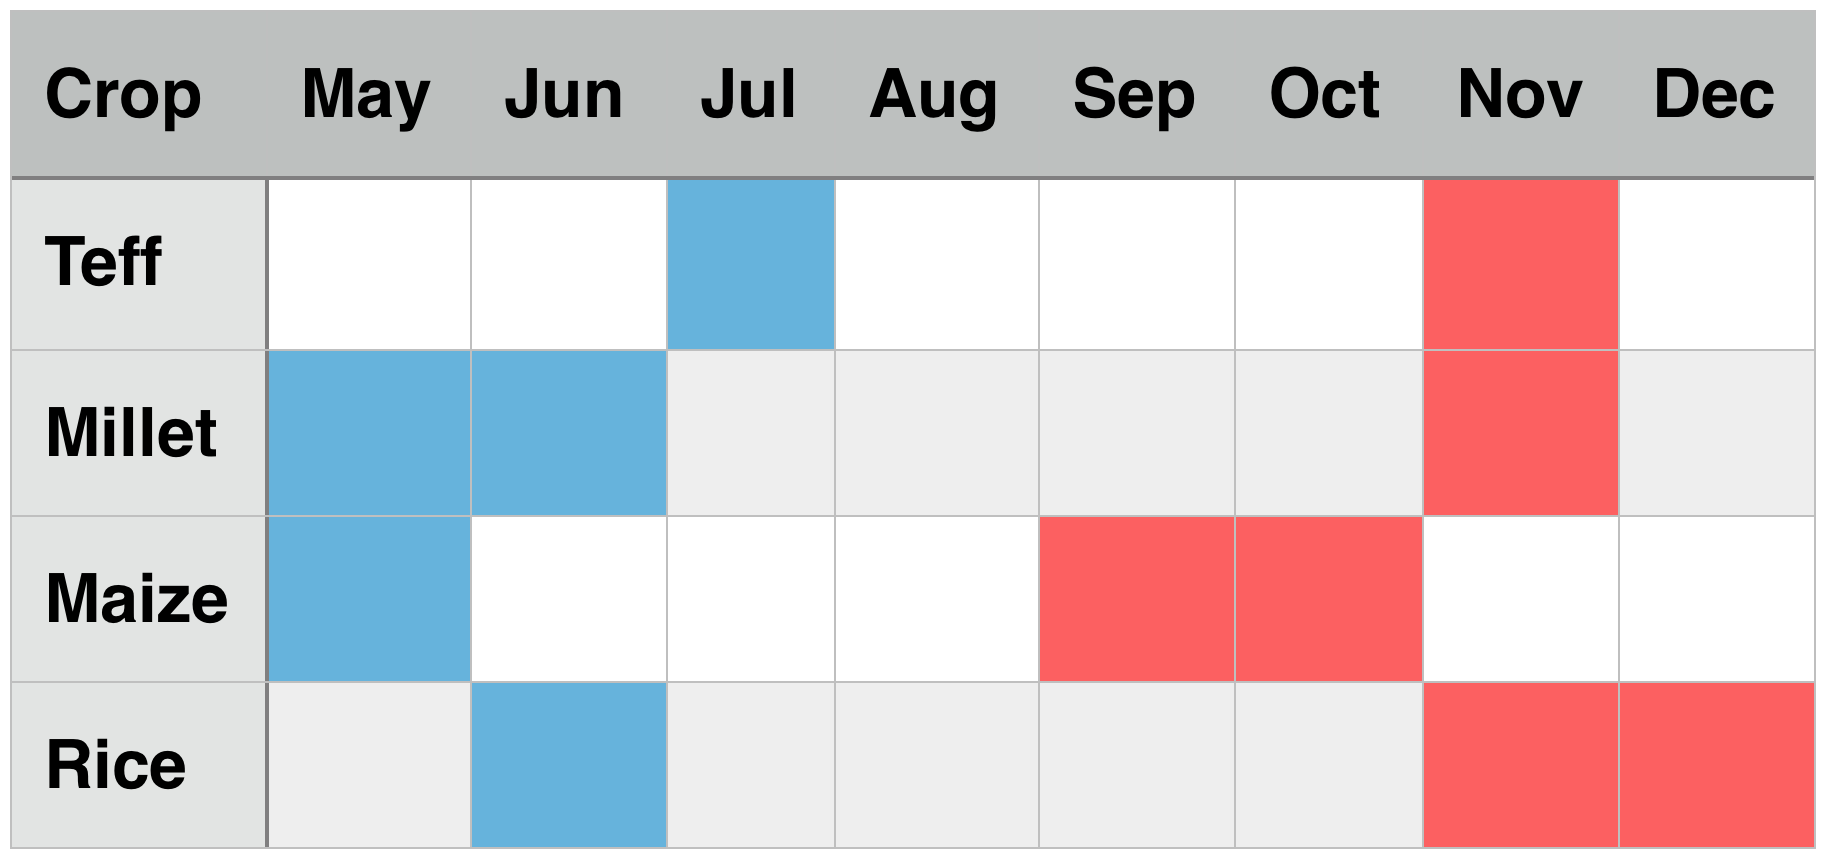
\includegraphics[width=0.6\textwidth]{./images/table1}
\end{center}
Key informants in Fogera described how rainfall patterns have become more irregular over the last two decades. Farmers we interviewed also indicated that the rain comes irregularly or at times, fails. There is a common agreement by farmers that years of sufficient rainfall, without hail or frost, providing good harvest have become less. Mostly increased variability and hazard are the new norm in recent decades \citep{wakjira2008diversifying}.\newline\linebreak
We data-mined public domain satellite data and produced water-related spatio-temporal domains that was then cross-referenced with informant’s accounts of water availability for the same space and time.\newline
}


%%%%%%%%%%%%%%%%%%%%%%%%%%%%%%%%%%%%%%%%%%%%%%%%%%%%%%%%%%%%%%%%%%%%%%%%%%%%%%%%
\blocknode{Rainfall deficit in May perceived as water scarcity}{
Farmers in upland Fogera associate the failure of the May rains with “drought”. For instance, a male farmer stated that, “When it is drought, it is the season of millet \& teff.” A female farmer stressed this seasonal scarcity in water availability by insisting that “It is this drought that hinders crop production.” However, if the rain fails in May, it does not necessarily represent an inevitable drought year, in that rain can be available in the subsequent months. Nevertheless, rainfed maize and millet planting in May is a central concern as it provides food and fodder for season, buffering household food security and reducing stress on further crop-related decision-making.\newline\linebreak
Rainfall variability has been one of the important factors impeding sustained implementation of intensification strategies, and particularly the use of fertilisers. Key informants indicated that rainfall variability has been discouraging the use of fertiliser due to risk of unsuccessful crop production which exacerbates farmers’ indebtedness besides losing production.\newline\linebreak
Vulnerability and capacity to respond to rainfall variability differs depending on individual natural, financial and social assets, as well as gender and socio-cultural variables. Farmers in Fogera have been attempting to respond to problems related to water availability based on adaptation, indigenous knowledge, practicing available options.\newline\linebreak
Responses undertaken by individual farmers and communities include: adjusting planting times and cropping pattern; deploying traditional ecological knowledge of soil to mitigate risk associated with water availability, expanding traditional and motor-pump irrigation \citep{dessalegn2014is}; and sponsoring religious figures to ameliorate the violation of spiritual sanctions that are transgressed in contemporary agricultural production.\newline
}

%%%%%%%%%%%%%%%%%%%%%%%%%%%%%%%%%%%%%%%%%%%%%%%%%%%%%%%%%%%%%%%%%%%%%%%%%%%%%%%%
\blocknode{Acknowledgements}{
\smallskip
\begin{tabular}{p{0.70\textwidth} c}
	The authors would like to acknowledge the CGIAR Research Program on Water, Land and Ecosystems (WLE ; \url{wle.cgiar.org}) Innovation Fund.
	&
	\hspace{3mm}
	\raisebox{-0.5\totalheight}{
\includegraphics[width=0.27\textwidth]{./images/WLE}}
\end{tabular}
}

\startthirdcolumn

%%%%%%%%%%%%%%%%%%%%%%%%%%%%%%%%%%%%%%%%%%%%%%%%%%%%%%%%%%%%%%%%%%%%%%%%%%%%%%%%
\blocknode{Spring Maize and food security}{
\begin{center}
	\begin{tabular}{ll}
 	\begin{tabular}{p{0.35\textwidth}}
Looking into the cumulative transpiration yearly signals (Figure 3), there is non uniformity, thus variations in water availability to vegetation. Following farmers' interviews and looking more closely into the April-June period, we found that in one case (figure 4), farmers perspective on the Spring maize crop sensitivity to variability of rainfall can be quantified in space and time by remote sensing cumulative transpiration. We found that crops were not transpiring enough by an amount of 20 to 50 mm during a period of about 20 days, depending on the type of year. Averaged on a daily basis, this means a crop transpiration gap of 1-2.5 mm/day. Such gap is small and can be artifically provided by temporary supplemental irrigation practices for example.\newline\linebreak
We argue that a better understanding of the dynamics of water variability and the implications on water management, agricultural production and livelihoods should consider small-holder farmers’ perceptions, concerns and responses. This is essential to devise well-targeted policies and interventions that can improve livelihoods, as well as optimising water management and agricultural production.\newline\linebreak
Cumulative transpiration on a yearly basis highlights different years, and heterogeneity periods (breaks) in the growing curve. Looking closely into the May-July period, one can identified the transpiration gap found most of the time for the early Maize crop much discussed by farmers. Out of 14 years, only 4 seem to have made the transpiration leap above the others (red ellipse in Figure 4). The leap can be quantified by an average of 20mm of rainfall over a period of 20 days, 1 mm of transpiration per day is missing at minimum (red ellipse) and 2.5mm/day at maximum (yellow ellipse) from mid-June to early July.
	\end{tabular}
 	& 
 	\begin{tabular}{c}
 	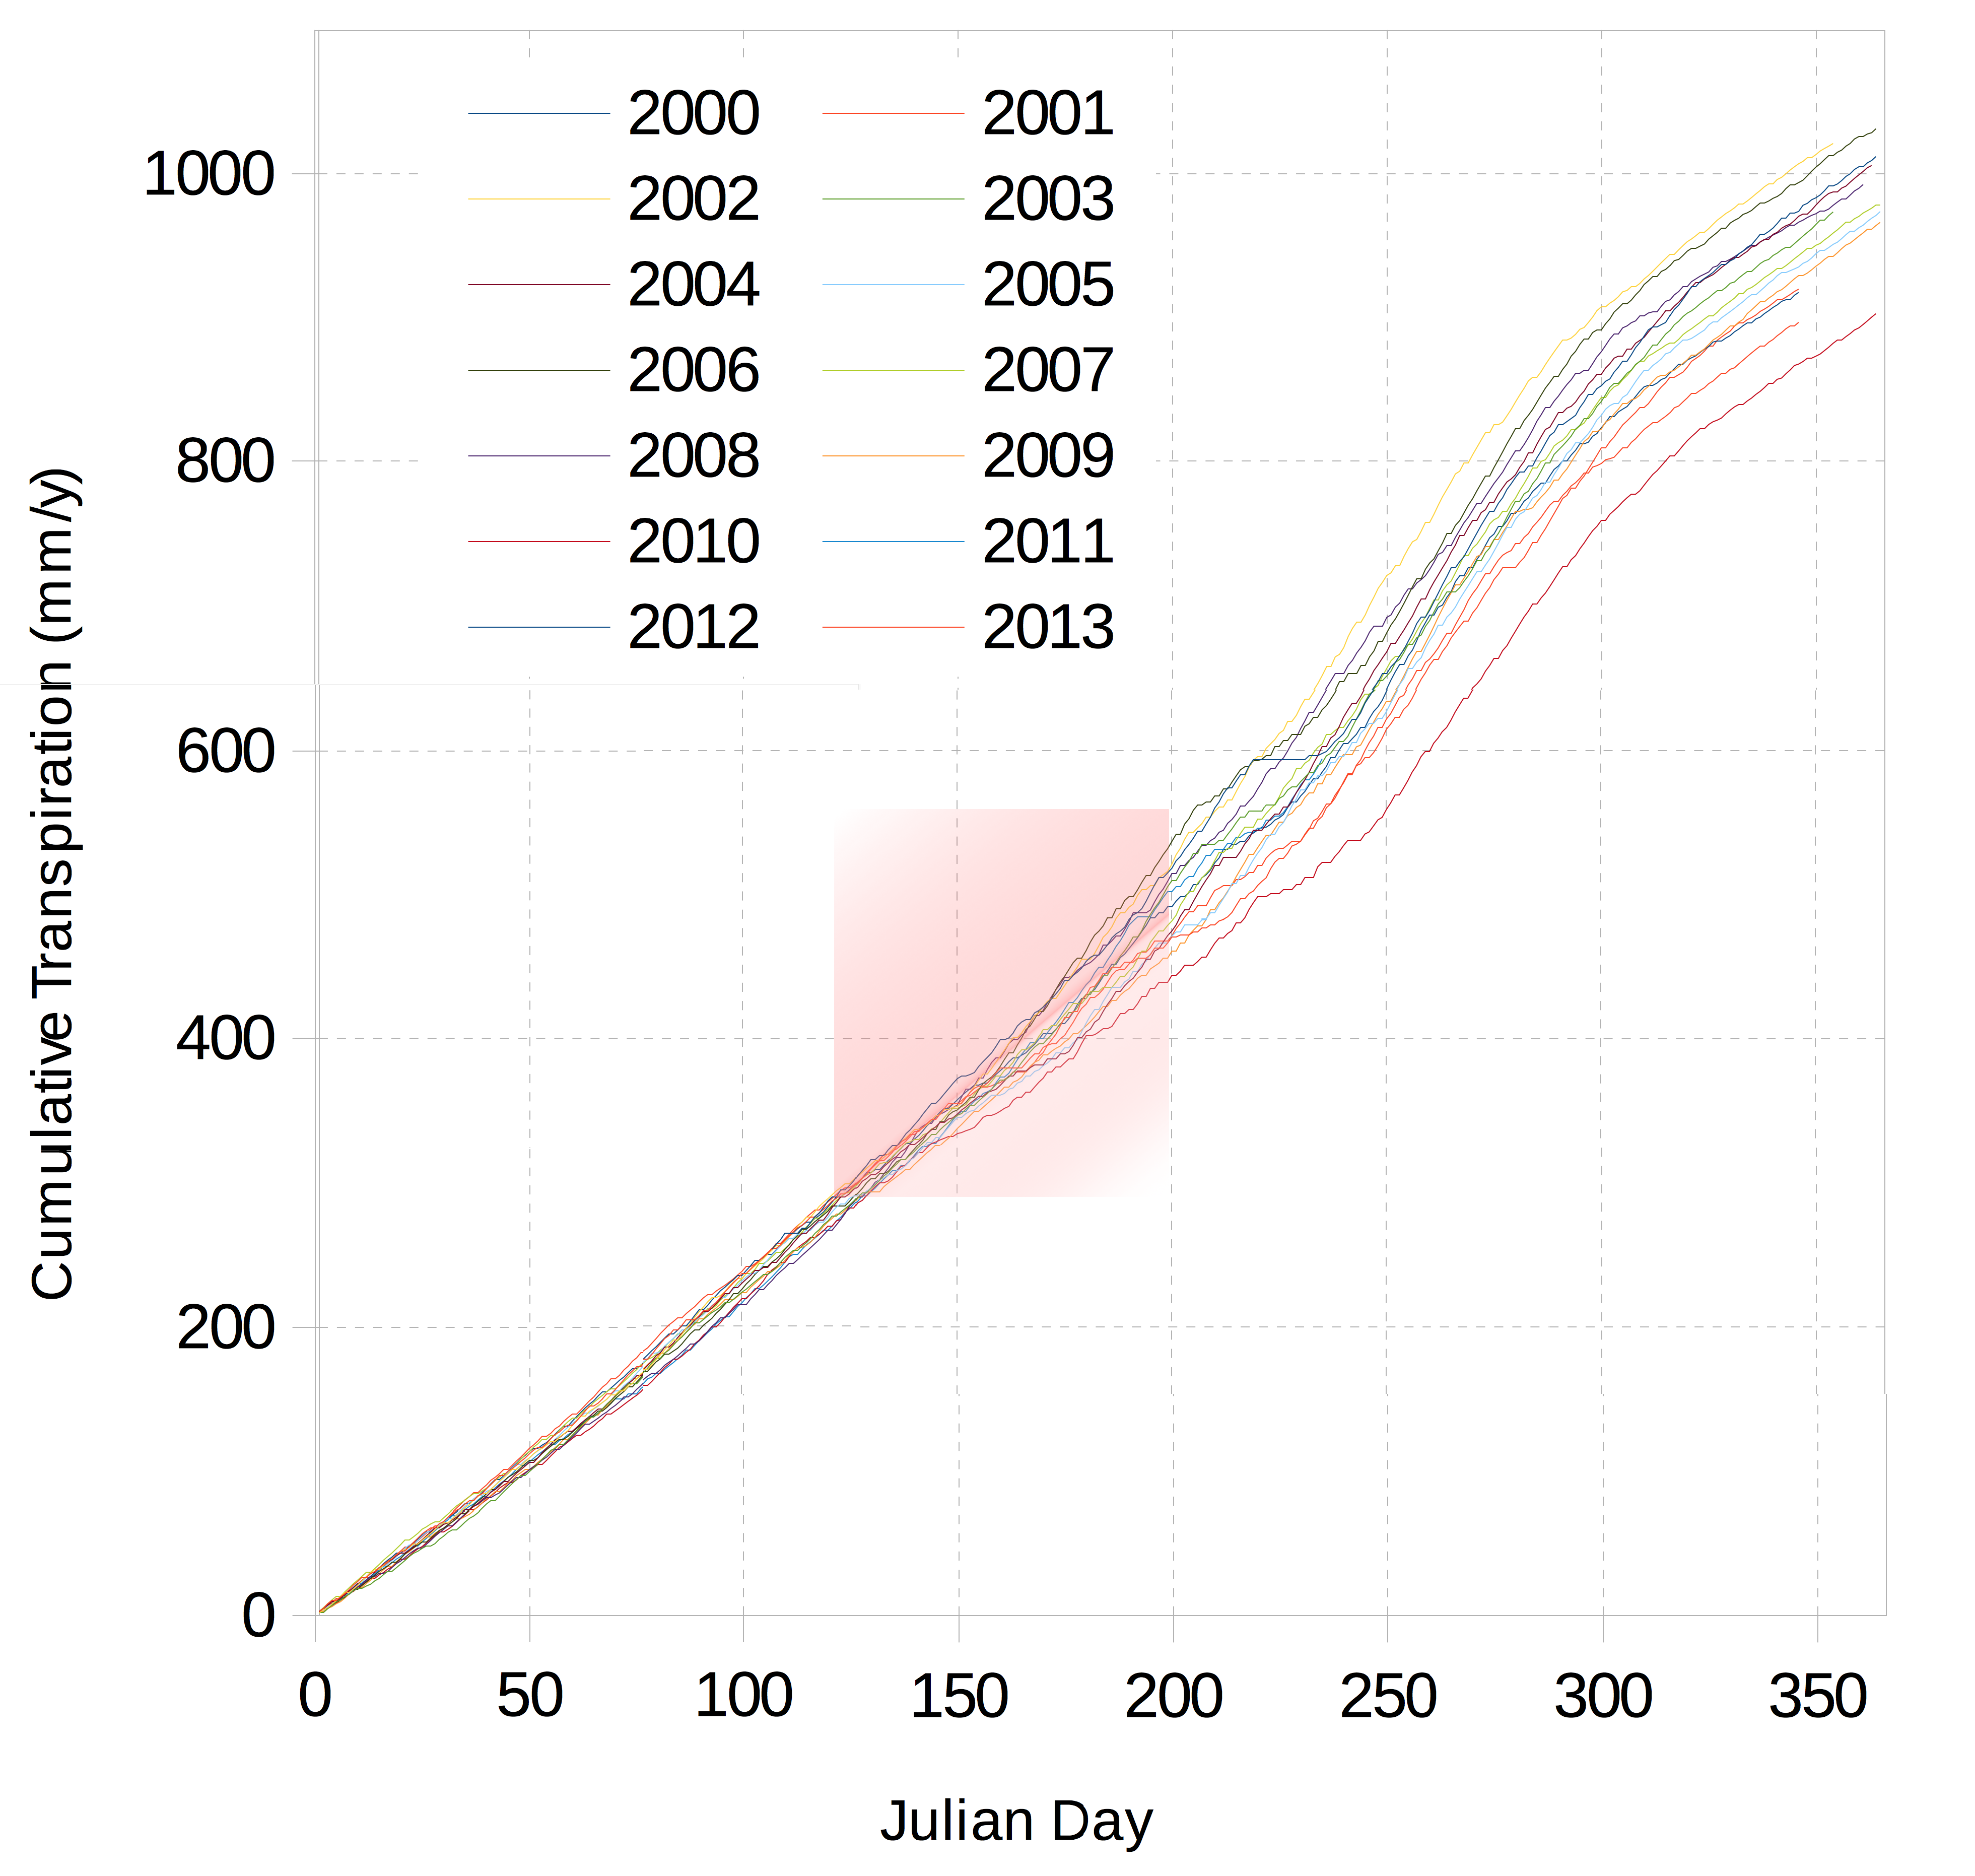
\includegraphics[width=0.55\textwidth]{./images/fig1big}\\
 	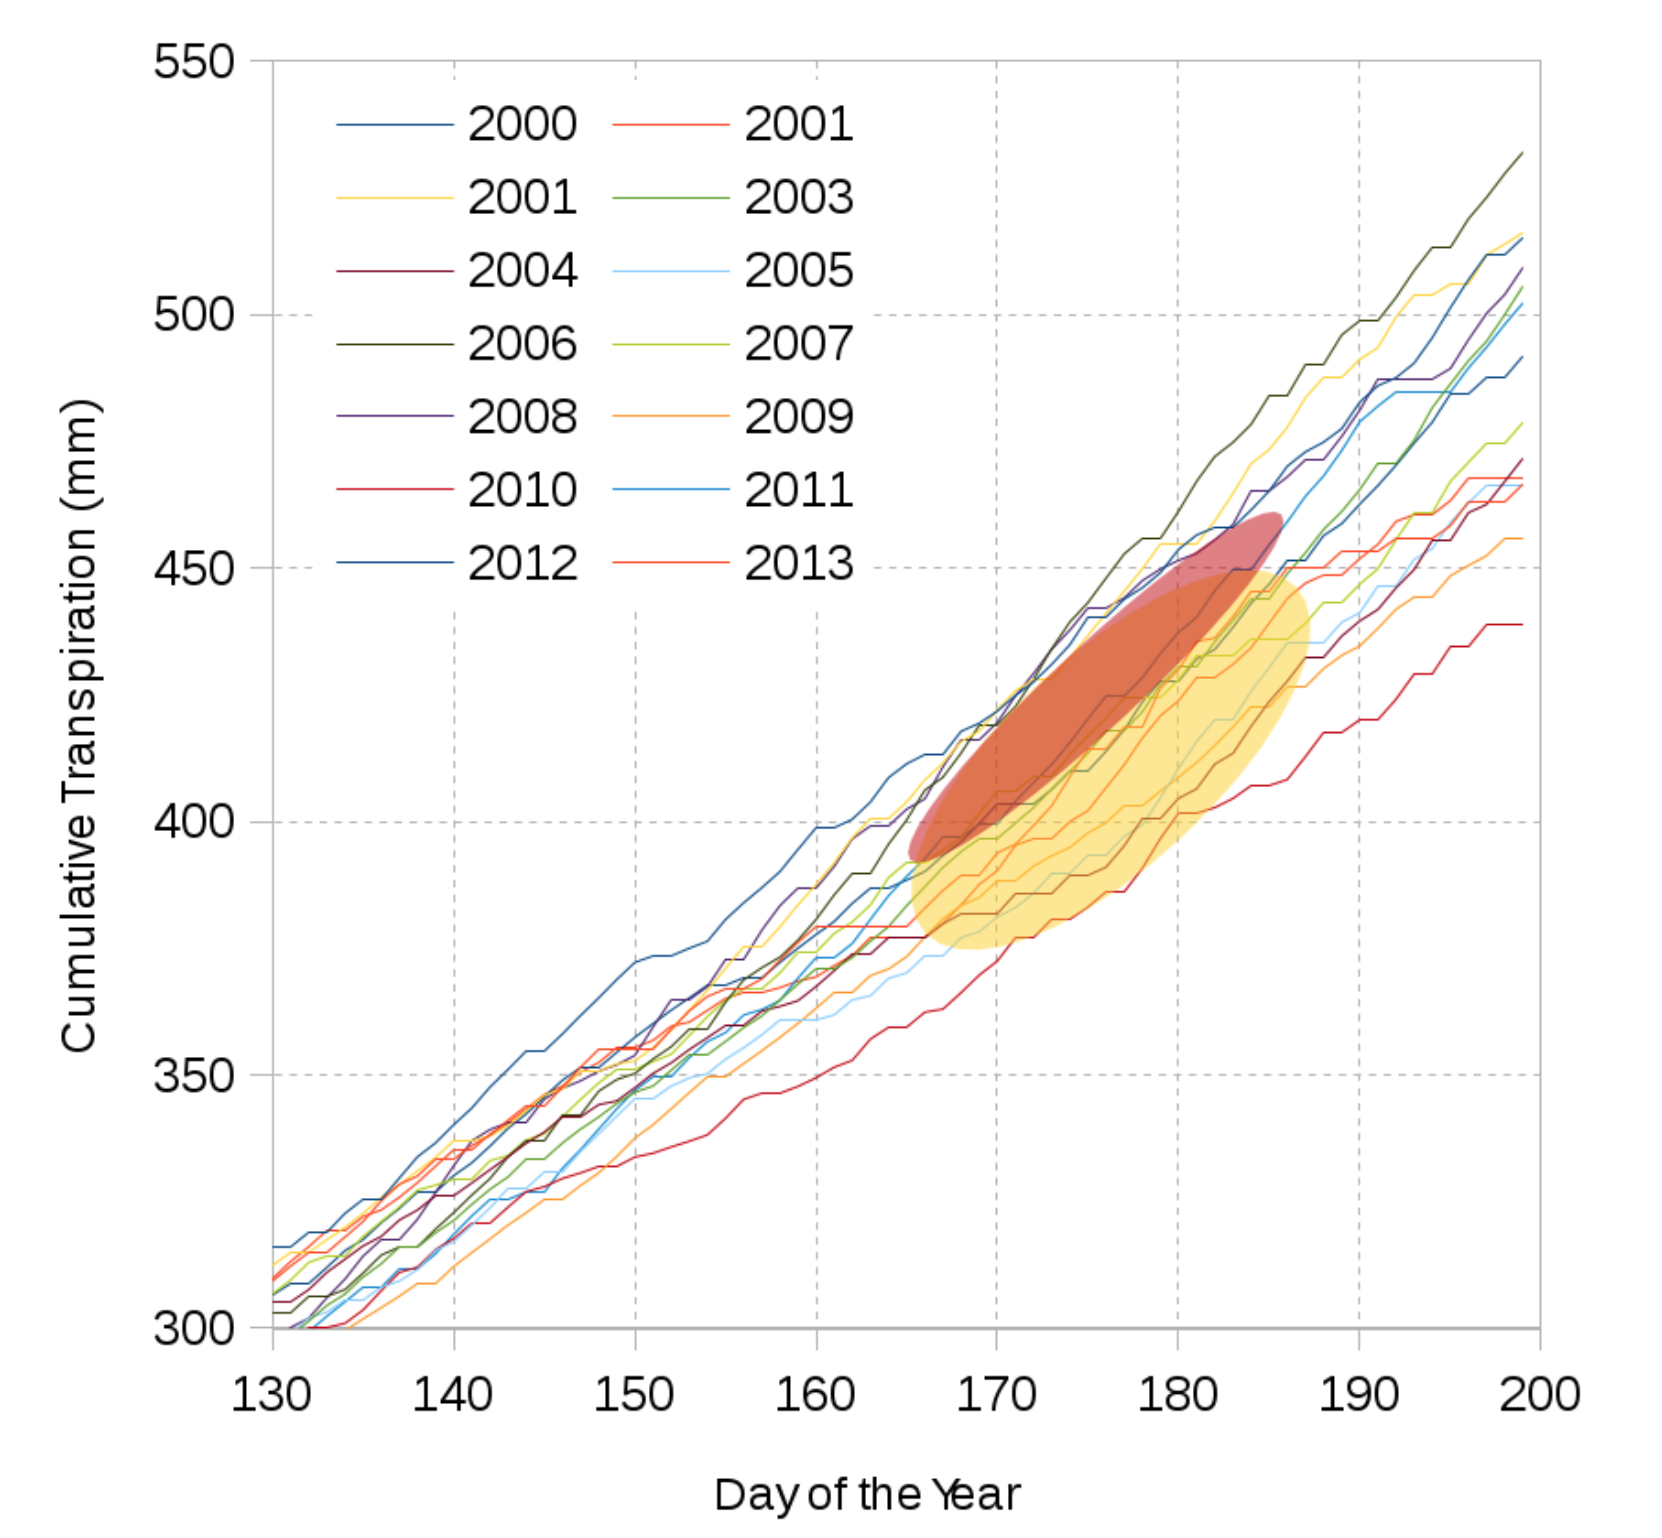
\includegraphics[width=0.55\textwidth]{./images/fig1}\\
	\end{tabular}
	\end{tabular}
	\vspace{5mm}
\end{center}
\begin{flushright}
Figure 3\&4: Cumulative transpiration per year \& month of May.\\
\end{flushright}

}

%%%%%%%%%%%%%%%%%%%%%%%%%%%%%%%%%%%%%%%%%%%%%%%%%%%%%%%%%%%%%%%%%%%%%%%%%%%%%%%%
\getcurrentrow{box}
\coordinate (funkcionalita) at (box.south west);
\coordinate (funkcionalitaeast) at (box.east);
\coordinate (screenshot) at (box.north west);

\blocknode{References}{
\small
\begingroup
\renewcommand{\section}[2]{}%
\bibliographystyle{plain}
\bibliography{poster}
\endgroup

\smallskip
\hrulefill
%\vspace{-5pt}

\begin{center}
\begin{tabular}{cp{0.9\textwidth}}
\begin{minipage}{0.15\textwidth}

\includegraphics[width=0.7in]{./images/iwmi_qr.pdf}
\end{minipage}

\begin{minipage}{0.3\textwidth}
\small {\url{www.iwmi.org}}
\end{minipage}

\begin{minipage}{0.15\textwidth}

\includegraphics[width=0.7in]{./images/grass_qr.pdf}
\end{minipage}

\begin{minipage}{0.3\textwidth}
\small {\url{grass.osgeo.org}}
\end{minipage}
\end{tabular}
\end{center}

\hrulefill
\vspace{14pt}
\begin{center}
\newcommand{\logowidth}{5em}
\newcommand{\logospace}{\hspace{0.1em}}
\noindent

\includegraphics[width=\logowidth]{./svg_images/public_domain_logo.pdf}
\raisebox{0.7\height}{\logospace 2015 GRASS Development Team}
\end{center}
}



\startfourthcolumn

%%%%%%%%%%%%%%%%%%%%%%%%%%%%%%%%%%%%%%%%%%%%%%%%%%%%%%%%%%%%%%%%%%%%%%%%%%%%%%%
\blocknode{Yearly Transpiration gap in the Upper Nile Basin}{
\smallskip
The Upper Nile Basin has a dramatic range of altitude from 483m reaching to 4517m at most. While most of the high altitude areas and various water bodies (in blue in Figure 4) are not or very less vegetated, the transpiration gap is relatively uninteresting. On the other hand, very clearly (in red in Figure 4), valleys are under deficit of transpiration from their potential level, vegetation is under stress.

\begin{center}
	\begin{tabular}{ll}
 	\begin{tabular}{c}
 	 \includegraphics[width=0.48\textwidth]{./images/Ta_Gap_2001}\\
 	 \includegraphics[width=0.48\textwidth]{./images/Ta_Gap_2006}
	\end{tabular}
 	& 
 	\begin{tabular}{c}
 	\includegraphics[width=0.48\textwidth]{./images/Ta_Gap_2011}\\
 	\includegraphics[width=0.48\textwidth]{./images/Ta_Gap_2014}
	\end{tabular}
	\end{tabular}
	Figure 4: Area Equalized Transpiration Gap in the Upper Nile Basin.\\
	\vspace{5mm}
 	\begin{tabular}{| c | c |}
	\hline
	&\\
	2001 & 2011\\
	&\\
	\hline
	&\\
	2006 & 2014\\
	&\\
	\hline
	\end{tabular}
\end{center}


This averaged daily deficit for a full year does not do justice to seasonal variations, but encompasses the potential for analysis of much longer temporal periodicity, we are only starting to decifer the monthly and yearly structures. It is clear at this point that Fogera woreda and one of its basin Gumura are a more common case than thought initially in terms of yearly transpiration gap budget.\newline 

}

%%%%%%%%%%%%%%%%%%%%%%%%%%%%%%%%%%%%%%%%%%%%%%%%%%%%%%%%%%%%%%%%%%%%%%%%%%%%%%%%
\blocknode{Conclusions}{
\smallskip
Space science as in remote sensing plant transpiration data and analysis, enables to quantify the lack of water consumption to reach a minimum Spring maize harvest. This knowledge potentially complements and augments farmer’s resilience and responsiveness to rainfall variability. In such marginal landscapes access to this information, and development of a coping mechanism, can mean the difference between seasonal hunger and food security.\newline\linebreak

Extending the exploration field of view to the Upper Nile Basin, we can see the Fogera woreda and its basin Gumura seem to have a fairly common yearly behaviour for watersheds. The lower section of the valleys seem to be consistently to have vegetation under water stress. Searching for monthly periodicity in the gap of transpiration is a subject of further studies.\newline

}




\end{tikzpicture}

\end{document}
